%&LaTeX

\section{The Z-Transform and Convolution}

This lab covers the z-transform, used to convert arbitrary digital
signals to the frequency domain. It also exercises the relationship
between a filter's transfer function and impulse response and how the
operations of multiplication and convolution, respectively, can be
used to compute a filter's output.

\subsection{The z-transform, Transfer Function, \& Impulse Response}

A discrete signal $x[n]$ has a z-transform $X(z)$ defined by the
following equation:
\[
X(z)=\sum_{n=0}^{\infty}x[n]z^{-n}
\]
With this definition lets investigate a feed forward filter with ten
coefficients, $\{b_0, b_1,\cdots, b_9\}$.  Recall that the
\block{Filter} and \block{Coeff.} blocks of J-DSP allow us to specify
a filter in terms of its \emph{coefficients}, but we can also define
it in terms of its \emph{transfer function}. Considering the $b_k$
coefficients of the feed forward filter, the \block{Filter} block
implements the transfer function:
\begin{equation}
  H(z) = \sum_{k=0}^{9} b_k z^{-k}
\end{equation}
In previous labs we have computed the transfer function using the
delays of the \emph{defining function}.  Mathematically, we were
actually taking the z-transform of the \emph{impulse response}!  In
this example, the impulse response is:
\begin{equation}
  h[n] = \sum_{k=0}^{9} b_k \delta[k]
\end{equation}
where $\delta[k]$ is the unit impulse and only has value at
$k$. $H(z)$ and $h[n]$ form a z-transform pair,
$h[n]\xleftrightarrow{z} H(z)$. It should now be obvious why
feedforward filters are also known as finite impulse response filters
-- their impulse response only has a \emph{finite} number of
values. To compute the output, $y[n]$, using the impulse response we
use \emph{convolution}. Namely, we \emph{convolve} the input, $x[n]$,
by the impulse response, $h[n]$,
\begin{equation}
  y[n] = x[n] \ast h[n]  = \sum_{k=0}^{9}x[k]h[n-k]
\end{equation}
Alternatively, we can compute a filter's output by multiplying the
transfer function by the z-transform of the input to yield the
z-transform of the output:
\begin{equation}
  Y(z) = H(z) X(z)
\end{equation}
From a practical point of view, of course, it makes more sense to
implement a filter in terms of its impulse response. However, for
filters with long impulse responses, it is sometimes more convenient
to represent them mathematically using the transfer function (which we
now know is just the z-transform of the impulse response!).  So, in
effect, the J-DSP blocks allow us to invert the z-transform of various
signals.

\subsection{Z-Transforms}

\paragraph{Step 1.1} On paper, compute the z-transform, $X(z)$, of
	\begin{equation}
		x[n] = \left\{
		\begin{array}{ll}
			(-1)^n & n \ge 0 \\
			0 & n < 0
		\end{array}\right.
	\end{equation}
	Note that this is an infinite geometric series. 
	% Hand in hard copy of your work.
	What are the locations of any pole(s) (roots of the denominator
	polynomial) or zero(s) (roots of the numerator polynomial)?


\paragraph{Step 1.2} Evaluate the frequency response of $X(z)$ from
	step~1.1, $X(z)\big{|}_{z=e^{j\hat{\omega}}}$. 
	% Hand in hard copy of your work. 
	What kind of filter is this?


\paragraph{Step 1.3} Consider the z-transform:
	\begin{equation}
	  X(z) = 1 - 2z^{-1} + 3z^{-3} - z^{-5}  
	\end{equation}
	Write the inverse z-transform, $x[n]$, as a table of values for
	corresponding $n$ values.


\subsection{Impulse Response}

\paragraph{Step 2.1} Consider a filter with a transfer function
	\begin{equation}
	H(z) = 1 + 5z^{-1} - 3z^{-2} + 2.5z^{-3} + 4z^{-8}  
	\end{equation}
	What is the defining equation for this filter, $y[n] = F(x[n])$?


\paragraph{Step 2.2} What is the output sequence of the filter of
	Step~2.1 when the input is $x[n] = \delta[n]$?


\paragraph{Step 2.3} The impulse response of a filter is $h[n] = x[n]
	+ 2x[n-1] + x[n-2] - x[n-3]$, or equivalently, $h[n]=\{1,2,1,-1\}$,
	$n=\{0, 1, 2, 3\}$. Determine the response of the system to the input
	signal $x[n]=\{1,2,3,1\}$, $n=\{0, 1,2,3\}$. Use J-DSP to check your
	results. Include an image of the J-DSP block diagram with plots of the
	\block{Sig Gen} signal and the filter output in your report.  Note
	that the \block{Sig Gen} block has a \emph{user-defined}
	\option{signal} option; use \button{reset} to reset all the signal
	values to zero before entering your own. Additionally, you can view
	the values in the \block{Plot} block.


\paragraph{Step 2.4} Change the input to the filter of Step~2.3 to be
	$\delta[n]$, using the \option{signal} set to ``Delta''. What are the
	output values? How do they compare to the impulse response? Include a
	plot of the filter output values in your report.


\begin{figure}[t] 
   \centering
   	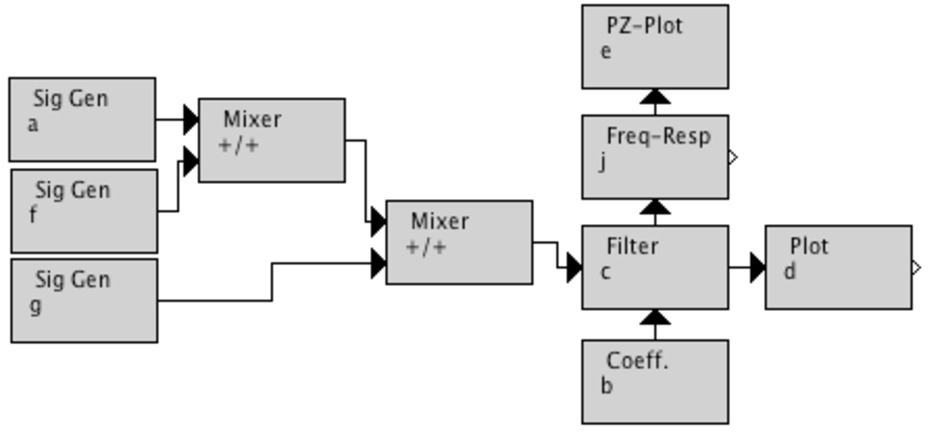
\includegraphics[width=4in]{lab6/threeinputproblem} 
   \caption{An example diagram for use in problem 2.5}
   \label{fg:threeinput}
\end{figure}
	
\paragraph{Step 2.5} Use J-DSP to determine the output of the filter \{1/3,1/3,1/3\}, $n=\{0,1,2\}$ for the
	input:
	\begin{equation}
	  x[n] = 4 + \sin[0.25\pi(n-1)] - 3 \sin[(2\pi/3)n]  
	\end{equation}
	An example diagram can be seen in Figure \ref{fg:threeinput}. Include an image 
	of the J-DSP block diagram with plots of the filter
	input and output in your report. Is the result expected? Why or why
	not?
	
	

\paragraph{Step 2.6} Create your own \block{UserDefinedFun} block to implement convolution in J-DSP. 
	To test your function, make sure it works exactly like the \block{Filter} block in J-DSP.
	Use the diagram in Figure \ref{fg:userdefined} to plot the difference between your function output and the \block{Filter} block output.
	Use the filter \{1/3,1/3,1/3\}, $n=\{0,1,2\}$ from step 2.5.
	Note: refer to section \ref{sec:example} for how to use the \block{UserDefinedFun} block in J-DSP.
	
	\begin{figure}[t]
	    \begin{center}	     
	        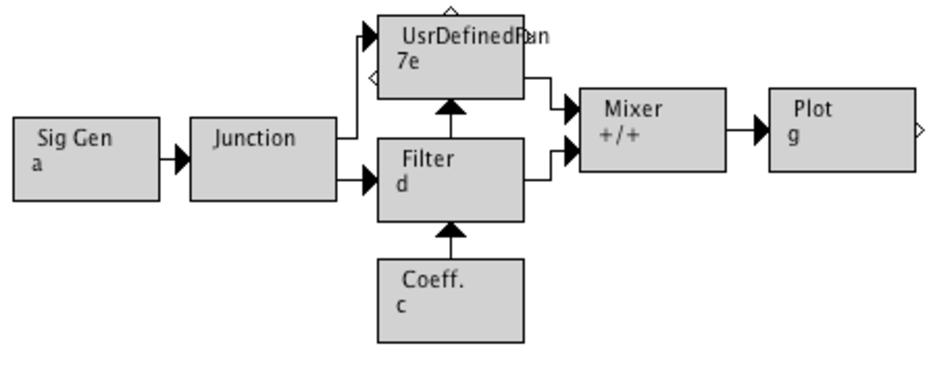
\includegraphics[width=4in]{lab6/userdefinedtest}
	        \caption{A diagram to plot the difference between \block{UserDefinedFun}
	         function output and the \block{Filter} block output for use in step 2.6.}
	         \label{fg:userdefined}
	    \end{center}
	  \end{figure}
	  
	  

\subsection{Canceling Sinusoidal Components}

Filters can be designed to cancel sinusoids.  Construct a filter in
J-DSP with the following impulse response:
\begin{equation}
h[n] = \delta[n] - 2\cos(\pi/4) \delta[n-1] + \delta[n-2]
\end{equation}

\paragraph{Step 3.1} Plot the frequency response for this filter. What
	are the zero locations?


\paragraph{Step 3.2} Use as an input to this filter the signal $x[n] =
	\sin\hat{\omega}n$, using the two frequencies $\hat{\omega} = \pi/2$
	and $\hat{\omega} = \pi/4$. Simulate the filter in J-DSP for each of
	these two inputs. Plot the filter output for each. When do we get
	cancellation?

\paragraph{Step 3.3} Can you modify the filter coefficients to cancel
	the other sinusoid? If so, show your work.


\subsection{Example User Defined J-DSP Function}\label{sec:example}
Open J-DSP and navigate to the \option{Advanced} function set. There
is one block called \block{UserDefinedFun}. Place it now and double
click to open the dialog.  You will see a dialog with example text for
a prototype java class.  In particular the class will look like:
\begin{lstlisting}
public void myCode(double[]x1,double[]x2, double[]y1, double[]y2,
		double[]b1,double[]a1, double[]b2, double[]a2, 
		double para1, double para2, double para3)
{
  //                            /\(3)
  //                --------------------           
  //           (0)<|                    |>(4)
  //               |      BLOCK         |    
  //           (1)<|                    |>(5)
  //                --------------------           
  //                            \/(2)

  // x1, x2 - input at pin 0 and pin1
  // y1, y2 - output at pin 4 and pin5
  // b1 - FIR Coefficients of the filter at input pin 2, 
  // a1 - IIR Coefficients of the filter at input pin 2
  // b2 - FIR Coefficients of the filter at output pin 3, 
  // a2 - IIR Coefficients of the filter at output pin 3

  // Para1, Para2 and Para3 are the variables that could be used 
  // in the code and can be controlled from the block Dialog.

  // Paste your code here
  // compile the file
  // upload the .class file
}
\end{lstlisting}
You can copy this code as a prototype and create your own signal
processing algorithms!  For now, you will mainly deal with the $x$ and
$y$ arrays. Each of the arrays is of length 256.  You can access this
like a any regular array in java, {\it x1.length=256}. We also have
access to four variable length arrays, {\it a1 a2 b1 b2} which contain
any filter coefficients as inputs or outputs to the function.

Lets start by creating our own .java file. Copy the example code on
the next page and save it as a .java file using your favorite java
text editor or plain text editor. The example code creates a weighted
sum of the entries in each index of {\it x1}. Namely, it goes through
each value of {\it x1} and uses the {\it b1} filter coefficients to
weight and sum the value into {\it y1}. Save the file as
``MyFunction1.java'' and then compile the file using your favorite
compiler tool for java (javac from the command line works fine for
linux and mac or The Java SE Development Kit 6 (JDK 6) can be used in
windows). This creates ``MyFunction1.class.''

After compiling, remember where you saved the ``MyFunction1.class''
compiled file. You will need to tell J-DSP where the file is
located. Go back to the J-DSP block diagram and press
\button{open}. Navigate to the ``MyFunction1.class'' compiled file and
press \option{open}. That's it! J-DSP will automatically use the
function when you attach inputs and outputs. To test the function we
just made you can connect a \block{SigGen} block to the top left pin
and a \block{Coeff} pin to the bottom as shown on page
\pageref{fg:userdefexample}. You should see a weighted sum of the
input when you plot the output. You should be able to change the
output by changing the weighting coefficients from \block{Coeff}. In
the example on page \pageref{fg:userdefexample} we are taking a
weighted sum (using the weights in {\it b1}) of each coefficient in
{\it x1} three times.  You are now ready to start developing your own
functions in J-DSP!

\begin{lstlisting} 
public class MyFunction1
{
  public void myCode(double[]x1,double[]x2, double[]y1, double[]y2,
      double[]b1,double[]a1, double[]b2, double[]a2, 
      double para1, double para2, double para3)
  {
    //                            /\(3)
    //                --------------------           
    //           (0)<|                    |>(4)
    //               |      BLOCK         |    
    //           (1)<|                    |>(5)
    //                --------------------           
    //                            \/(2)
		
    // x1, x2 - input at pin 0 and pin1
    // y1, y2 - output at pin 4 and pin5
    // b1 - FIR Coefficients of the filter at input pin 2, 
    // a1 - IIR Coefficients of the filter at input pin 2
    // b2 - FIR Coefficients of the filter at output pin 3, 
    // a2 - IIR Coefficients of the filter at output pin 3
		
    // Para1, Para2 and Para3 are the variables that could be used 
    // in the code and can be controlled from the block Dialog.
		
    for( int i = 0 ; i < 256 ; i++)
    {
      y2[i] = 0;
      for(int j=0 ; j < b1.length ; j++)
      {
        y2[i] += x1[i]*b1[j];
      }
			
    }
    // Paste your code here
    // compile the file
    // upload the .class file
  }
}
\end{lstlisting}

 \begin{figure}[h]
    \begin{center}     
        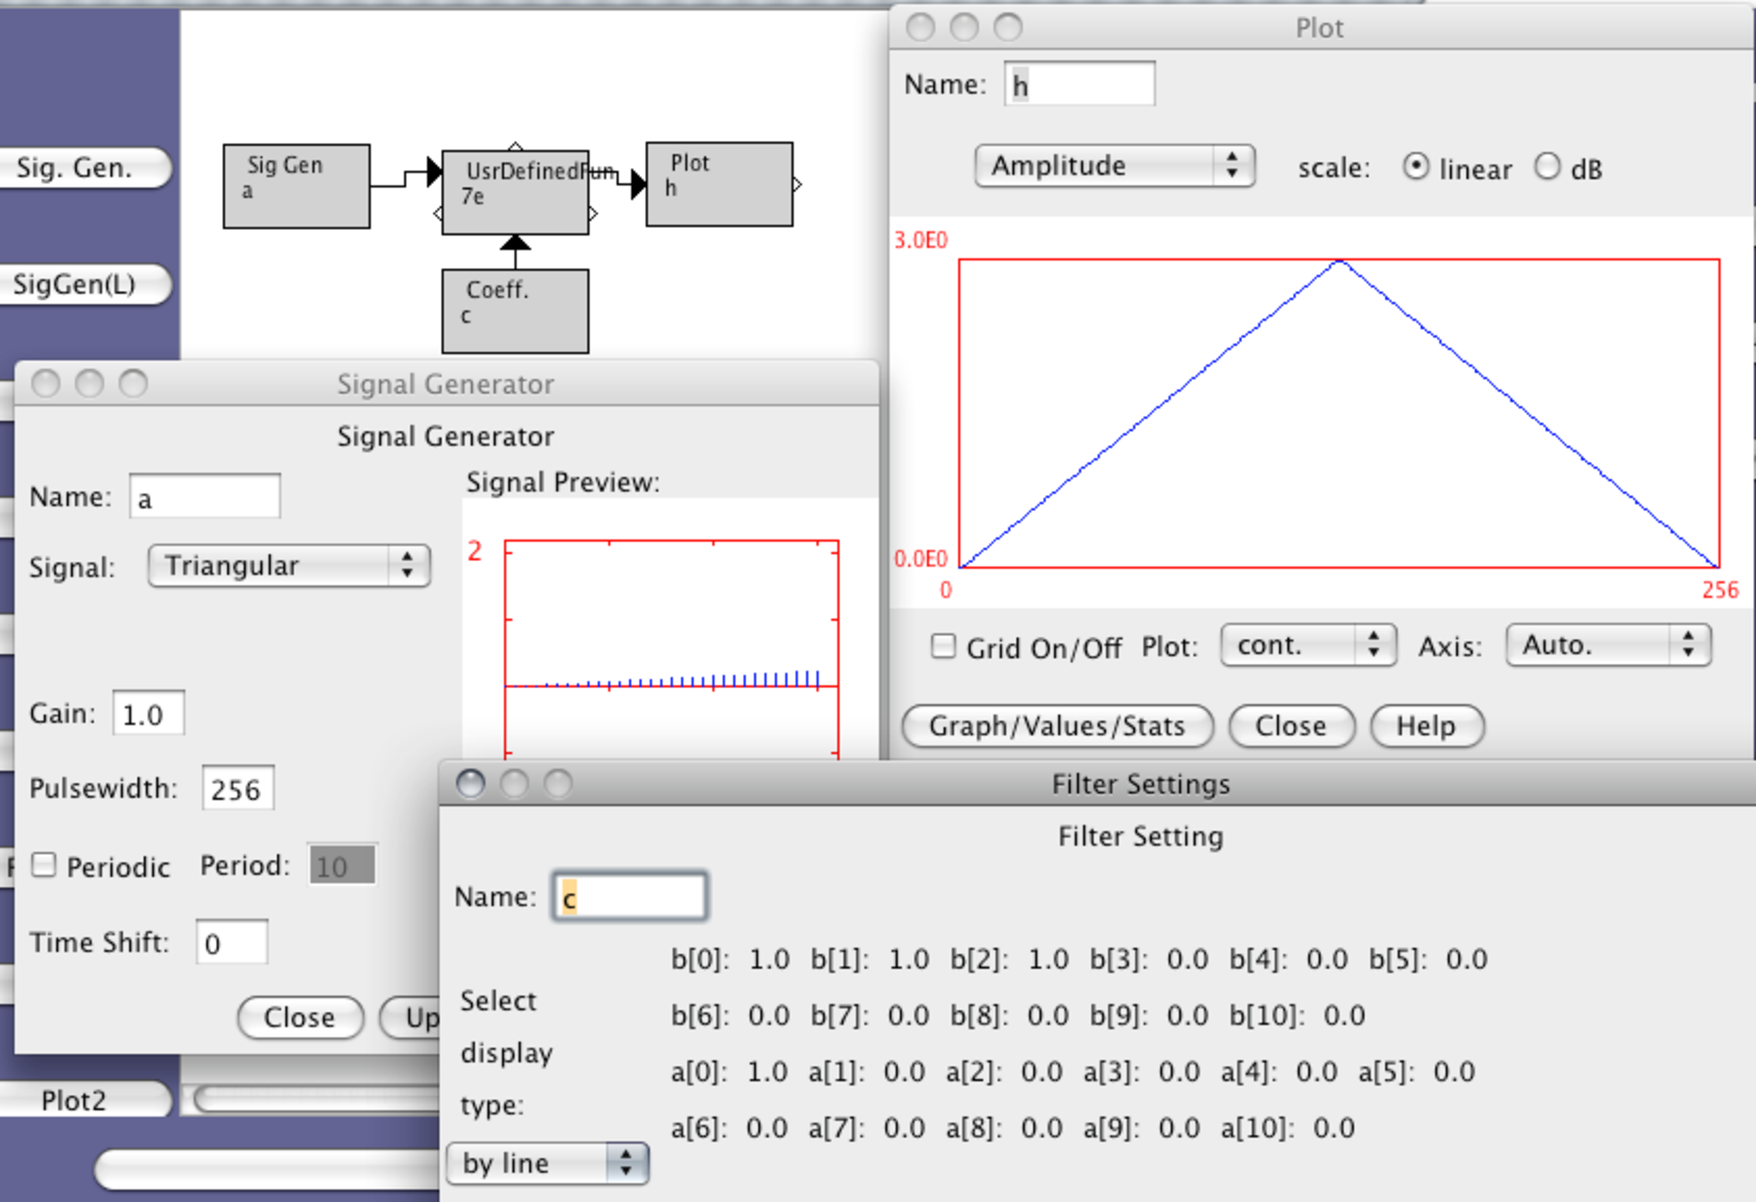
\includegraphics[width=6in]{lab6/function1examplewithplot}
        \caption{The result of using the weighted sum example code in J-DSP.}
    \end{center}
    \label{fg:userdefexample}
  \end{figure}

\subsection{Bonus: More $z$-Transforms and Convolutions}

The following properties of the $z$-transform may be useful here:

\begin{center}
\begin{tabular}{|l|c|c|} \hline
Property      & Time Domain, $Z^{-1}\{\cdot\}$ & z-Domain, $Z\{\cdot\}$ \\ \hline\hline
Linearity     & $a_1x[n]+a_2y[n]$ & $a_1X(z)+a_2Y(z)$\\ 
Time shift    & $x[n-k]$       & $z^{-k}X(z)$\\ 
Scaling in the z-domain 
              & $a^nx[n]$        & $X(a^{-1}z)$ \\ 
Time reversal & $x[-n]$        & $X(z^{-1})$\\ 
Differentiation in the z-domain 
              & $nx[n]$          & $-z \deriv{X(z)}{z}$ \\ 
Convolution   & $x[n] \ast y[n]$       & $X(z)Y(z)$ \\ \hline
\end{tabular}
\end{center}



\paragraph{$z$-Transform of arbitrary sequences}
Give the $z$-transform of the following sequences, $x[n]$ (assume
$x[n]=0$ for all $n$ not stated):
\begin{enumerate}
\item $x[n]=\{2, 4, 6, 4, 2\}$, $n = \{0, 1, 2, 3, 4\}$

\item $x[n] = \delta[n]$

\item $x[n] = \delta[n-1]$

\item $x[n] = 2\delta[n] - 3\delta[n-1] +4\delta[n-3]$

\item $x[n] = 2\delta[n] + 4\delta[n-1] + 6\delta[n-2] + 4\delta[n-3] + 2\delta[n-4]$
\end{enumerate}


\paragraph{Inverse $z$-transforms}
Give the inverse $z$-transform of $H(z) = 1 + 5z^{-1} - 3z^{-2} +
2.5z^{-3} +4z^{-8}$.

\paragraph{Transfer function \& impulse response}
Give the transfer function and impulse response for a filter with
zeros at $(r, \hat{\omega}) = \{(1, 0), (1, \pm \pi/2), (0.9, \pm
\pi/3)\}$.

% LocalWords:  WebQ MATLAB DSP
